% Provenance (never printed): see sources/outline_sources.md (Year 2: ancient massifs,
% Caledonian and Variscan belts; the Wilson cycle; supercontinents). Caledonian phases after
% McKerrow, Mac Niocaill and Dewey (2000) and Schiffer et al. (2020); the Wilson cycle after
% Chenin et al. (2018) and Schiffer et al. (2020); the Variscan belt after Faure (2024);
% supercontinents after Nance (2022); Siccar Point after the IUGS Geoheritage description.
% Model ocean and supercontinent chart from figdata/bachelor-2/wilson.py. Exercise and problem
% values in the Book 4 scratch calculator calc/ch15.py.
\chapter{Masif Tua dan Siklus Wilson}\label{ch:b2:wilson-cycle}

Di pantai tenggara Skotlandia, di Siccar Point, lapisan-lapisan batu pasir kelabu berdiri tegak
di bawah tudung batu pasir merah yang miring landai ke arah laut. Lapisan kelabu itu diendapkan di
sebuah samudra pada awal Silur, lalu terlipat dan terbelah ketika samudra itu menutup; lapisan itu terkikis
menjadi permukaan yang tidak rata; pada Devon Akhir, kerikil merah menimbunnya, dan pembentukan pegunungan kedua
yang lebih lemah lalu memiringkan lapisan merah itu. Satu tebing merekam sebuah samudra yang telah
lenyap, sebuah sabuk pegunungan yang telah hilang, dan sabuk berikutnya. Bab ini membaca rekaman semacam itu,
menghimpunnya menjadi siklus yang diikuti cekungan samudra, dan mundur selangkah untuk melihat irama terpanjang
dari semuanya, yaitu penyatuan dan pemecahan \omterm{def:b2:wilson-cycle:supercontinent}{superbenua}.
% ledger: iugs:siccar-orogenies, iugs:siccar-point

\begin{recall}
\textbf{Dari volume-volume sekolah}: Pangea dan pemecahannya, \omterm{def:b2:wilson-cycle:supercontinent}{superbenua}; ketidakselarasan;
laju denudasi, pantulan isostatik, dan peluruhan eksponensial jajaran pegunungan yang terkikis
oleh sungai-sungainya. \textbf{Dari volume Tahun 1}: celah benua, tepi pasif, dan
punggungan tengah samudra, laju pemekaran penuh dan setengah; subduksi dan tepi aktif.
\textbf{Dari \cref{ch:b2:crustal-melting} sampai \cref{ch:b2:himalaya-andes}}: \omterm{def:b2:crustal-melting:migmatite}{migmatit} dan
granit; \omterm{def:b2:alpine-orogen:orogen}{orogen}, \omterm{def:b2:alpine-orogen:ophiolite}{ofiolit}, sutura, \omterm{def:b2:alpine-orogen:nappes}{nappe}, \omterm{def:b2:alpine-orogen:foreland}{flysch} dan \omterm{def:b2:alpine-orogen:foreland}{molasse}, \omterm{def:b2:alpine-orogen:foreland}{cekungan depan-pegunungan}; \omterm{def:b2:himalaya-andes:types}{orogen tumbukan} dan
\omterm{def:b2:himalaya-andes:types}{orogen tipe Andes}; \omterm{def:b2:himalaya-andes:thickening}{penebalan kerak}, tebal Airy, dan \omterm{def:b2:himalaya-andes:collapse}{keruntuhan gravitasi}.
\end{recall}

\begin{omfigure}
\centering
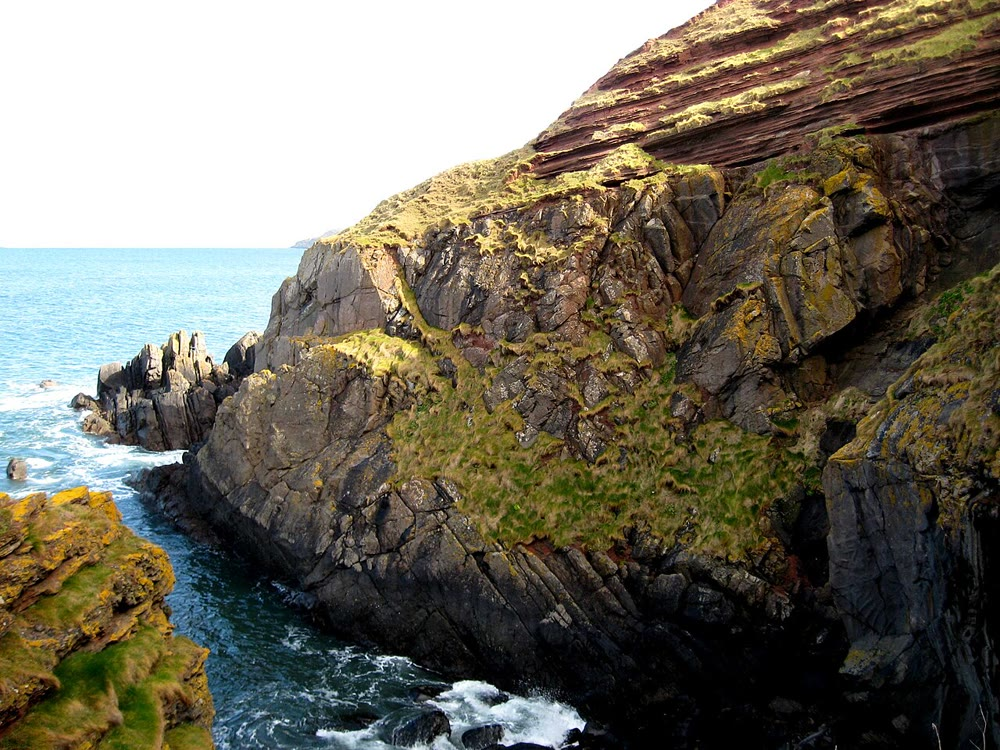
\includegraphics[width=0.64\linewidth]{images/book4/b2-15-siccar-point.jpg}
\par\smallskip{\small Siccar Point, dilihat dari tenggara tanjung: lapisan-lapisan greywacke Silur kelabu yang hampir
tegak, terlipat dalam orogenesis Kaledonia, di bawah lapisan merah Devon Atas yang miring
landai. Foto: dave souza, 2008, CC BY-SA 4.0.}
\end{omfigure}
% ledger: iugs:siccar-orogenies

\section{Sabuk yang terkikis sampai akarnya}\label{sec:b2:wilson-cycle:old}

Eropa Barat dan Amerika Utara bagian timur dilintasi sabuk-sabuk pegunungan yang jauh lebih tua daripada
Alpen. Puncak-puncaknya telah hilang, tetapi batuannya tetap ada. Tiga di antaranya penting di sini.

Sabuk \emph{Kaledonia} membentang dari Norwegia melalui Skotlandia dan Irlandia sampai Newfoundland dan
Appalachia utara, dan berlanjut melalui Greenland Timur dan Svalbard. Sabuk ini adalah rekaman sebuah
samudra, Iapetus, yang pada Paleozoikum awal terletak di antara Laurentia, leluhur Amerika
Utara dan Greenland, di barat laut, serta Baltica dan Avalonia di tenggara dan timur.
Tepi-tepinya telah terbelah sekitar 600 juta tahun yang lalu; penutupannya, dari Kambrium sampai
Devon, menghasilkan serangkaian tumbukan, sehingga orogenesis Kaledonia mencakup sekitar
200 juta tahun. Istilah itu menamai sebuah tempat dan sebuah samudra, bukan suatu zaman.
% ledger: mckerrow00:caledonian, schiffer20:caledonides

Sabuk \emph{Variscan}, yang dalam teks lama disebut Hercynia, melintasi Eropa dari barat daya
Inggris dan Belgia melalui Prancis dan Iberia sampai Eropa tengah; sabuk \emph{Appalachia} di
Amerika Utara bagian timur adalah kembaran baratnya. Bersama-sama, keduanya merekam penutupan samudra-samudra
di antara benua selatan, Gondwana, dan benua utara, yang baru saja disatukan oleh
tumbukan-tumbukan Kaledonia. Tumbukan terakhirnya, pada Karbon Akhir dan Perm, meninggalkan
sabuk lipatan yang membentang timur--barat melalui Eropa selatan dan timur laut--barat daya di antara
Amerika Utara bagian timur dan Afrika barat laut, dan bersamanya \omterm{def:b2:wilson-cycle:supercontinent}{superbenua} Pangea.
% ledger: schiffer20:variscan, faure24:variscan

Bagaimana orang mengenali sabuk pegunungan yang telah tererosi selama tiga ratus juta tahun?
Tidak dari reliefnya, yang telah hilang. Orang mencari bagian-bagiannya, yang masing-masing telah dijumpai
pada bab-bab sebelumnya:
\begin{itemize}
\item \emph{sutura} yang dijajari \emph{\omterm{def:b2:alpine-orogen:ophiolite}{ofiolit}}, irisan-irisan dasar samudra yang menutup;
\item sabuk \emph{batuan metamorf}, sering berderajat tinggi, yaitu akar kerak yang menebal,
yang kini berada di permukaan karena kilometer-kilometer di atasnya telah tererosi;
\item \emph{granit} dan \emph{\omterm{def:b2:crustal-melting:migmatite}{migmatit}}, hasil pelelehan kerak yang dibawa oleh
penebalan dan pemanasan;
\item sedimen samudra yang menutup dan sedimen sabuk itu: \emph{\omterm{def:b2:alpine-orogen:foreland}{flysch}} yang tercurah ke cekungan dalam
selama konvergensi, \emph{\omterm{def:b2:alpine-orogen:foreland}{molasse}} yang tercurah ke \omterm{def:b2:alpine-orogen:foreland}{cekungan depan-pegunungan} dan cekungan antargunung;
\item \emph{ketidakselarasan sudut}, tempat lapisan yang lebih muda bertumpu di atas lapisan yang telah terlipat dan
tererosi sebelumnya, yang memberi umur deformasi di antara keduanya.
\end{itemize}

\begin{definition}[Peneplain]\label{def:b2:wilson-cycle:peneplain}
Yang disebut \emph{peneplain}\index{peneplain} adalah permukaan daratan berelief rendah, di dekat aras dasar
erosi, yang memotong batuan dengan kekerasan dan struktur yang berbeda-beda melalui erosi panjang atas suatu
relief lama.
\end{definition}

Sabuk Variscan adalah \omterm{def:b2:alpine-orogen:orogen}{orogen} yang panas. Di Alpen \cref{ch:b2:alpine-orogen}, batuannya
mengikuti gradien metamorfik sekitar \qty{8}{\celsius} per kilometer; di sabuk Variscan,
sekitar \qty{30}{\celsius} per kilometer. Keraknya meleleh secara luas: di Masif Sentral Prancis
dan Masif Armorika, \omterm{def:b2:crustal-melting:migmatite}{migmatit} terbentuk antara sekitar 330 dan 325 juta tahun yang lalu, dan
granit menerobosnya. Pelelehan itulah perbedaan utamanya dengan Alpen Barat. Ketika
tumbukan berakhir, kerak yang menebal menipis oleh ekstensi, batuan metamorf terangkat
di sepanjang bidang lepasan, dan cekungan antargunung membuka; lalu erosi meratakan jajaran itu menjadi
\omterm{def:b2:wilson-cycle:peneplain}{peneplain} Perm dan Trias tempat sedimen siklus berikutnya diendapkan.
% ledger: faure24:variscan

\begin{omfigure}
\centering\small
\begin{tabular}{>{\raggedright\arraybackslash}p{0.2\linewidth}|>{\raggedright\arraybackslash}p{0.17\linewidth}|>{\raggedright\arraybackslash}p{0.52\linewidth}}
fase & umur & apa yang bertumbukan \\ \hline
Penobscot & 490--485 Ma & busur kepulauan yang tersesar-dorong ke atas tepi Avalonia \\
Grampian, Taconic & 480--455 Ma & busur kepulauan dan Laurentia (di Skotlandia dan Appalachia utara) \\
Shelve & awal Ordovisium Akhir & Avalonia dan Baltica; Laut Tornquist menutup \\
Skandia & 425--400 Ma & Baltica dan Laurentia; \omterm{def:b2:alpine-orogen:nappes}{nappe-nappe} besar Skandinavia \\
Acadia & Devon Awal & \omterm{def:b2:wilson-cycle:terrane}{terrane} dari Gondwana dan benua baru; Iapetus menutup \\
\end{tabular}
\par\smallskip{\small Fase-fase utama orogenesis Kaledonia. Fase-fase awal adalah
tumbukan busur dengan busur atau dengan benua, fase-fase akhir adalah tumbukan benua; sebagian besar
fase dimulai pada waktu yang berbeda di tempat yang berbeda.}
\end{omfigure}
% ledger: mckerrow00:phases, schiffer20:caledonides

Tabel Kaledonia di atas menunjukkan tanda lain sabuk tua: sabuk itu bersifat komposit. Sebelum
kedua benua bertemu, busur-busur dan blok-blok yang lebih kecil datang satu per satu dan disatukan.

\begin{definition}[Terrane; mikrobenua]\label{def:b2:wilson-cycle:terrane}
Yang disebut \emph{terrane}\index{terrane} adalah blok kerak yang dibatasi sesar, yang sejarah geologinya
berbeda dari sejarah tetangganya, dan yang terbawa ke posisinya sekarang oleh gerakan lempeng; terrane dapat
berupa busur kepulauan, plato samudra, irisan dasar samudra, atau kepingan benua. Yang disebut
\emph{mikrobenua}\index{mikrobenua} adalah blok kerak benua, yang lebih kecil daripada
benua, yang terpisah dari benua-benua oleh kerak samudra.
\end{definition}

Avalonia adalah blok semacam itu: sejalur kerak yang meninggalkan tepi Gondwana, membuka Samudra
Rheic di belakangnya pada Ordovisium, menyeberangi Iapetus, dan merapat pada Baltica, lalu
Laurentia. Armorika dan Saxothuringia, yang kini berada di Prancis dan Jerman, menyusulnya berturut-turut;
sutura-suturanya, yang ditandai \omterm{def:b2:alpine-orogen:ophiolite}{ofiolit}, membagi sabuk Variscan menjadi zona-zona dari daratan depan utara
di benua utara lama sampai daratan depan selatan di Gondwana.
% ledger: schiffer20:caledonides, schiffer20:variscan, faure24:variscan

\begin{omfigure}
\centering
\begin{tikzpicture}[x=0.5cm, y=0.5cm, font=\scriptsize]
\tikzset{cont/.style={fill=orange!25, draw=black!60, line width=0.4pt},
  terr/.style={fill=orange!45, draw=black!60, line width=0.4pt},
  ocn/.style={font=\scriptsize\itshape, text=blue!50!black},
  belt/.style={pattern=north east lines, pattern color=red!60!black, draw=red!60!black}}
% panel A
\begin{scope}
\fill[blue!6] (0,0) rectangle (9,8);
\draw[cont] (0.3,4.2) -- (3.0,4.0) -- (3.4,7.7) -- (0.3,7.7) -- cycle;
\node[align=center] at (1.7,6.0) {Lau-\\rentia};
\draw[cont] (6.0,5.4) -- (8.7,5.0) -- (8.7,7.7) -- (6.4,7.7) -- cycle;
\node at (7.4,6.6) {Baltica};
\draw[cont] (0.3,0.3) -- (8.7,0.3) -- (8.7,1.6) -- (0.3,1.9) -- cycle;
\node at (4.5,0.95) {Gondwana};
\draw[terr] (3.8,2.4) -- (6.6,2.2) -- (6.6,2.9) -- (3.8,3.1) -- cycle;
\node at (5.2,2.65) {Avalonia};
\node[ocn] at (4.6,5.4) {Iapetus};
\node[ocn] at (7.7,2.55) {Rheic};
\node[anchor=north west, font=\small\bfseries] at (0.1,8.9) {A: sekitar 480 Ma};
\end{scope}
% panel B
\begin{scope}[xshift=5.0cm]
\fill[blue!6] (0,0) rectangle (9,8);
\draw[cont] (0.3,3.6) -- (3.0,3.4) -- (3.4,7.7) -- (0.3,7.7) -- cycle;
\draw[cont] (3.0,3.4) -- (3.4,7.7) -- (8.7,7.7) -- (8.7,4.4) -- (5.2,4.6) -- (5.0,3.4) -- cycle;
\draw[terr] (3.0,3.4) -- (5.0,3.4) -- (5.2,4.6) -- (8.7,4.4) -- (8.7,3.6) -- (3.0,2.8) -- cycle;
\draw[red!60!black, line width=1.2pt] (3.0,3.4) -- (3.4,7.7);
\draw[red!60!black, line width=1.2pt] (5.0,3.4) -- (5.2,4.6) -- (8.7,4.4);
\node[align=center] at (1.6,5.6) {Lau-\\rentia};
\node at (6.6,5.7) {Baltica};
\node at (6.4,3.75) {Avalonia};
\node at (6.0,7.1) {\textbf{Laurussia}};
\draw[cont] (0.3,0.3) -- (8.7,0.3) -- (8.7,1.3) -- (0.3,1.5) -- cycle;
\node at (4.5,0.8) {Gondwana};
\draw[terr] (2.2,1.9) -- (3.6,1.9) -- (3.6,2.3) -- (2.2,2.3) -- cycle;
\draw[terr] (5.0,1.8) -- (6.6,1.8) -- (6.6,2.2) -- (5.0,2.2) -- cycle;
\node[ocn] at (7.7,2.3) {Rheic};
\node[anchor=north west, font=\small\bfseries] at (0.1,8.9) {B: sekitar 420 Ma};
\end{scope}
% panel C
\begin{scope}[xshift=10.0cm]
\fill[blue!6] (0,0) rectangle (9,8);
\draw[cont] (0.3,3.0) -- (8.7,3.0) -- (8.7,7.7) -- (0.3,7.7) -- cycle;
\draw[cont] (0.3,0.3) -- (8.7,0.3) -- (8.7,3.0) -- (0.3,3.0) -- cycle;
\fill[belt] (0.3,2.5) -- (8.7,2.5) -- (8.7,3.5) -- (0.3,3.5) -- cycle;
\node[fill=orange!25, inner sep=1pt] at (4.5,5.6) {Laurussia};
\node[fill=orange!25, inner sep=1pt] at (4.5,1.3) {Gondwana};
\node[fill=white, fill opacity=0.85, text opacity=1, inner sep=1pt, align=center] at (4.5,3.0)
  {sabuk Variscan--Appalachia};
\node[ocn] at (7.6,0.7) {};
\node[anchor=north west, font=\small\bfseries] at (0.1,8.9) {C: sekitar 300 Ma, Pangea};
\end{scope}
\end{tikzpicture}
\par\smallskip{\small Tiga saat penutupan samudra Iapetus dan Rheic, berupa
sketsa skematis tanpa proyeksi peta dan tanpa skala: posisi, ukuran, dan bentuk hanya
bersifat topologis. A: Avalonia telah meninggalkan Gondwana dan Samudra Rheic membuka di belakangnya. B: Iapetus telah
menutup; Laurentia, Baltica, dan Avalonia membentuk Laurussia, di sepanjang sutura Kaledonia (garis merah);
blok-blok yang lebih kecil sedang menyeberangi Samudra Rheic. C: Gondwana telah bertemu Laurussia di sepanjang
sabuk Variscan--Appalachia (berarsir).}
\end{omfigure}
% ledger: mckerrow00:caledonian, mckerrow00:phases, schiffer20:caledonides, schiffer20:variscan, faure24:variscan

\section{Siklus Wilson}\label{sec:b2:wilson-cycle:cycle}

Pada 1966, J. Tuzo Wilson bertanya apakah Atlantik pernah menutup lalu
membuka kembali. Fosil-fosil Paleozoikum awal dan tengah memberitahunya bahwa sebuah samudra yang luas pernah
memisahkan fauna Amerika Utara dari fauna Eropa Barat, samudra yang tidak lagi
ada dari Paleozoikum akhir sampai pertengahan Mesozoikum. Atlantik modern telah membuka
hampir di tempat samudra yang lebih tua itu, Iapetus, menutup.
% ledger: schiffer20:wilson, chenin18:cycle

\begin{definition}[Siklus Wilson]\label{def:b2:wilson-cycle:wilson}
Yang disebut \emph{siklus Wilson}\index{siklus Wilson} adalah urutan tahap yang dilalui suatu
cekungan samudra untuk membuka dan menutup kembali di antara tepi-tepi benua: pembentukan celah benua,
pemisahan dan pemekaran dasar laut, samudra yang melebar dengan tepi pasif, awal
subduksi, menyempit dan menutupnya samudra, tumbukan benua, serta keruntuhan
dan erosi sabuk, setelah itu benua yang telah menyatu dapat terbelah lagi di sepanjang zona yang sama.
\end{definition}

Gambar di bawah mengikuti tahap-tahap itu. Tahap-tahap itu adalah isi bab-bab sebelumnya yang disusun berurutan:
celah dan tepi pasif volume Tahun 1, tepi aktif dan busurnya,
tumbukan Alpen dan Himalaya, \omterm{def:b2:himalaya-andes:collapse}{keruntuhan gravitasi} Tibet, dan pengikisan lambat
sabuk-sabuk tua.

\begin{omfigure}
\centering
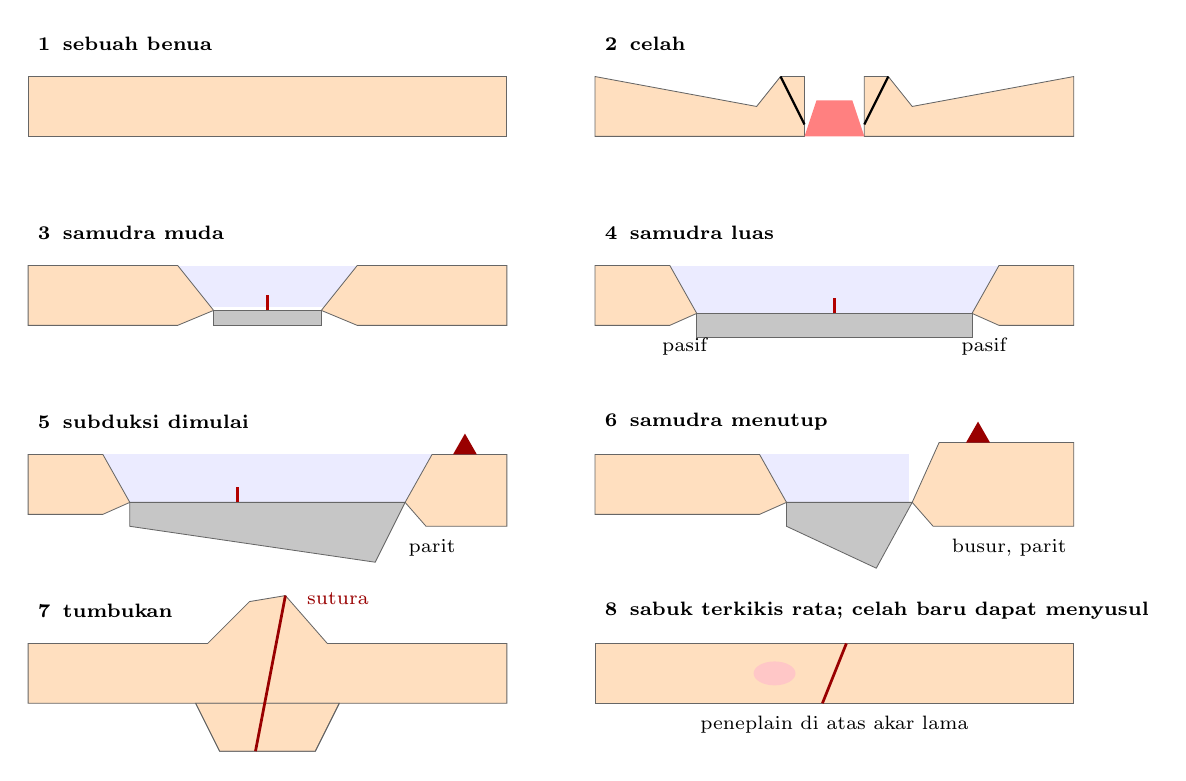
\begin{tikzpicture}[x=0.38cm, y=0.38cm, font=\scriptsize]
\tikzset{crust/.style={fill=orange!25, draw=black!60, line width=0.3pt},
  ocrust/.style={fill=gray!45, draw=black!60, line width=0.3pt},
  sea/.style={fill=blue!8},
  ttl/.style={anchor=west, font=\scriptsize\bfseries}}
% 1 continent
\begin{scope}
\draw[crust] (0,0) -- (16,0) -- (16,2) -- (0,2) -- cycle;
\node[ttl] at (0,3.1) {1\enspace sebuah benua};
\end{scope}
% 2 rift
\begin{scope}[xshift=7.2cm]
\draw[crust] (0,0) -- (7,0) -- (7,2) -- (6.2,2) -- (5.4,1.0) -- (0,2) -- cycle;
\draw[crust] (9,0) -- (16,0) -- (16,2) -- (10.6,1.0) -- (9.8,2) -- (9,2) -- cycle;
\fill[red!50] (7,0) -- (9,0) -- (8.6,1.2) -- (7.4,1.2) -- cycle;
\draw[thick] (6.2,2) -- (7,0.4); \draw[thick] (9.8,2) -- (9,0.4);
\node[ttl] at (0,3.1) {2\enspace celah};
\end{scope}
% 3 young ocean
\begin{scope}[yshift=-2.4cm]
\fill[sea] (5,2) -- (11,2) -- (11,0.6) -- (5,0.6) -- cycle;
\draw[crust] (0,0) -- (5,0) -- (6.2,0.5) -- (5,2) -- (0,2) -- cycle;
\draw[crust] (16,0) -- (11,0) -- (9.8,0.5) -- (11,2) -- (16,2) -- cycle;
\draw[ocrust] (6.2,0.5) -- (9.8,0.5) -- (9.8,0) -- (6.2,0) -- cycle;
\draw[red!70!black, thick] (8,0.5) -- (8,1.0);
\node[ttl] at (0,3.1) {3\enspace samudra muda};
\end{scope}
% 4 wide ocean
\begin{scope}[xshift=7.2cm, yshift=-2.4cm]
\fill[sea] (2.5,2) -- (13.5,2) -- (13.5,0.4) -- (2.5,0.4) -- cycle;
\draw[crust] (0,0) -- (2.5,0) -- (3.4,0.4) -- (2.5,2) -- (0,2) -- cycle;
\draw[crust] (16,0) -- (13.5,0) -- (12.6,0.4) -- (13.5,2) -- (16,2) -- cycle;
\draw[ocrust] (3.4,0.4) -- (12.6,0.4) -- (12.6,-0.4) -- (3.4,-0.4) -- cycle;
\draw[red!70!black, thick] (8,0.4) -- (8,0.9);
\node[anchor=north] at (3,-0.1) {pasif};
\node[anchor=north] at (13,-0.1) {pasif};
\node[ttl] at (0,3.1) {4\enspace samudra luas};
\end{scope}
% 5 subduction begins
\begin{scope}[yshift=-4.8cm]
\fill[sea] (2.5,2) -- (13.5,2) -- (13.5,0.4) -- (2.5,0.4) -- cycle;
\draw[crust] (0,0) -- (2.5,0) -- (3.4,0.4) -- (2.5,2) -- (0,2) -- cycle;
\draw[crust] (16,-0.4) -- (13.3,-0.4) -- (12.6,0.4) -- (13.5,2) -- (16,2) -- cycle;
\draw[ocrust] (3.4,0.4) -- (12.6,0.4) -- (11.6,-1.6) -- (3.4,-0.4) -- cycle;
\fill[red!60!black] (14.2,2) -- (14.6,2.7) -- (15.0,2) -- cycle;
\draw[red!70!black, thick] (7,0.4) -- (7,0.9);
\node[anchor=north] at (13.5,-0.5) {parit};
\node[ttl] at (0,3.1) {5\enspace subduksi dimulai};
\end{scope}
% 6 ocean closes
\begin{scope}[xshift=7.2cm, yshift=-4.8cm]
\fill[sea] (5.5,2) -- (10.5,2) -- (10.5,0.4) -- (5.5,0.4) -- cycle;
\draw[crust] (0,0) -- (5.5,0) -- (6.4,0.4) -- (5.5,2) -- (0,2) -- cycle;
\draw[crust] (16,-0.4) -- (11.3,-0.4) -- (10.6,0.4) -- (11.5,2.4) -- (16,2.4) -- cycle;
\draw[ocrust] (6.4,0.4) -- (10.6,0.4) -- (9.4,-1.8) -- (6.4,-0.4) -- cycle;
\fill[red!60!black] (12.4,2.4) -- (12.8,3.1) -- (13.2,2.4) -- cycle;
\node[anchor=north west] at (11.6,-0.5) {busur, parit};
\node[ttl] at (0,3.1) {6\enspace samudra menutup};
\end{scope}
% 7 collision
\begin{scope}[yshift=-7.2cm]
\draw[crust] (0,0) -- (16,0) -- (16,2) -- (10,2) -- (8.6,3.6) -- (7.4,3.4) -- (6,2) -- (0,2) -- cycle;
\fill[crust] (5.6,0) -- (10.4,0) -- (9.6,-1.6) -- (6.4,-1.6) -- cycle;
\draw[black!60, line width=0.3pt] (5.6,0) -- (6.4,-1.6) -- (9.6,-1.6) -- (10.4,0);
\draw[red!60!black, line width=1pt] (8.6,3.6) -- (7.6,-1.6);
\node[anchor=west, text=red!60!black] at (9.0,3.5) {sutura};
\node[ttl] at (0,3.1) {7\enspace tumbukan};
\end{scope}
% 8 worn flat
\begin{scope}[xshift=7.2cm, yshift=-7.2cm]
\draw[crust] (0,0) -- (16,0) -- (16,2) -- (0,2) -- cycle;
\draw[red!60!black, line width=1pt] (8.4,2) -- (7.6,0);
\fill[pink!60!red!40] (6.0,1.0) ellipse (0.7 and 0.4);
\node[anchor=north] at (8,-0.1) {peneplain di atas akar lama};
\node[ttl] at (0,3.1) {8\enspace sabuk terkikis rata; celah baru dapat menyusul};
\end{scope}
\end{tikzpicture}
\par\smallskip{\small Tahap-tahap \omterm{def:b2:wilson-cycle:wilson}{siklus Wilson}, berupa penampang skematis (tidak berskala):
kerak benua berwarna jingga, kerak samudra berwarna kelabu, punggungan berwarna merah, dan gunung api busur berupa
segitiga; pada panel terakhir, sutura dan sebuah granit tertinggal dalam kerak dengan tebal normal.}
\end{omfigure}
% ledger: chenin18:cycle, schiffer20:wilson

\subsection{Seberapa lebar, seberapa lama?}

Samudra tumbuh melalui pemekaran dasar laut di punggungannya dan menyusut melalui subduksi di parit-paritnya.
Pembukuan sederhana memberikan lebarnya.

\begin{proposition}[Lebar samudra sepanjang satu siklus]\label{prop:b2:wilson-cycle:width}
Misalkan sebuah samudra membuka pada waktu $t_0$ dan melebar dengan laju pemekaran penuh $V_s$ punggungannya, sampai
zona subduksi dimulai di salah satu tepi pada waktu $t_1$ dan menghabiskan dasar samudra dengan laju $V_c$
relatif terhadap tepi itu, dengan $V_c > V_s$, sementara punggungan masih memekar. Lebarnya adalah
\[
  W(t) = V_s\,(t - t_0) \quad (t_0 \le t \le t_1), \qquad
  W(t) = V_s\,(t_1 - t_0) - (V_c - V_s)\,(t - t_1) \quad (t \ge t_1),
\]
terbesar pada $t_1$, dan samudra menutup dalam waktu $V_s(t_1 - t_0)/(V_c - V_s)$ setelah subduksi
dimulai. Dengan pemekaran simetris, punggungan bergerak ke arah parit dengan laju $V_c - V_s/2$.
\end{proposition}

\begin{proof}
Anggaplah tepi yang memiliki parit tetap. Sebelum $t_1$, kedua tepi memisah dengan laju pemekaran
penuh $V_s$, sehingga lebarnya tumbuh dengan laju $V_s$ dari nol. Setelah $t_1$, lempeng di antara
parit dan punggungan bergerak ke arah parit dengan laju $V_c$; punggungan menambahkan $V_s$ pada jarak
antara lempeng itu dan lempeng jauh, sehingga tepi jauh bergerak ke arah parit dengan laju $V_c - V_s$,
yaitu laju berkurangnya lebar. Lebarnya mencapai nol setelah $V_s(t_1 - t_0)/(V_c -
V_s)$. Dengan pemekaran simetris, punggungan bergerak dengan rata-rata kecepatan lempeng di
kedua sisinya, $(V_c + (V_c - V_s))/2 = V_c - V_s/2$.
\end{proof}

Gambar di bawah memainkan pembukuan ini untuk samudra model bertipe Iapetus: pemekaran sejak
\qty{570}{Ma} dengan laju \qty{30}{mm} per tahun, subduksi sejak \qty{490}{Ma} yang menghabiskan \qty{60}{mm} per
tahun. Laju-laju itu adalah asumsi, nilai bulat seukuran yang terukur kini di samudra-samudra;
Iapetus yang sebenarnya tidak sesederhana itu dan tidak dikenal sebaik itu. Samudra model itu mencapai \qty{2400}{km}
dan menutup pada \qty{410}{Ma}, di dalam rentang waktu tumbukan Skandia.
% values (wilson.py): max_width_km 2400, closure_Ma 410; ledger: mckerrow00:caledonian, schiffer20:caledonides

\begin{omfigure}
\centering
% figdata/bachelor-2/wilson.py part ocean (model values: assumptions)
\begin{tikzpicture}
\begin{axis}[width=0.8\linewidth, height=5.0cm, x dir=reverse, xmin=360, xmax=600, ymin=0,
  ymax=3300, ytick={0,1000,2000,3000}, xlabel={umur (\unit{Ma})}, ylabel={lebar samudra (\unit{km})},
  tick label style={font=\scriptsize}, label style={font=\small}, xtick={600,560,...,360}]
\addplot[omThm, line width=1.2pt] table[x=t_Ma, y=width_km] {figdata/out/bachelor-2-wilson-ocean.dat};
\draw[dashed, black!50] (axis cs:490,0) -- (axis cs:490,2400);
\draw[dashed, black!50] (axis cs:570,0) -- (axis cs:570,2750);
\draw[dashed, black!50] (axis cs:410,0) -- (axis cs:410,2750);
\node[font=\scriptsize, anchor=south] at (axis cs:570,2750) {pemekaran dimulai};
\node[font=\scriptsize, anchor=south west] at (axis cs:488,2400) {subduksi dimulai};
\node[font=\scriptsize, anchor=south] at (axis cs:410,2750) {tumbukan};
\node[font=\scriptsize, anchor=west, align=left] at (axis cs:540,600) {membuka\\dengan laju $V_s$};
\node[font=\scriptsize, anchor=south west, align=left] at (axis cs:446,1150) {menutup\\dengan laju\\$V_c - V_s$};
\end{axis}
\end{tikzpicture}
\par\smallskip{\small Lebar sebuah samudra model sepanjang satu \omterm{def:b2:wilson-cycle:wilson}{siklus Wilson}, dari
\cref{prop:b2:wilson-cycle:width} dengan $V_s = \qty{30}{mm}$ per tahun sejak \qty{570}{Ma} dan $V_c
= \qty{60}{mm}$ per tahun sejak \qty{490}{Ma}. Waktu berjalan dari kiri ke kanan.}
\end{omfigure}

\subsection{Membuka di tempat menutup}

Gagasan Wilson bertumpu pada gagasan mekanis: sabuk tua adalah zona lemah, dan benua yang
ditarik terpisah cenderung patah di sepanjang zona-zona lemahnya, bukan menembus bagian dalamnya yang kuat dan
stabil.

\begin{definition}[Reaktivasi struktur]\label{def:b2:wilson-cycle:reactivation}
Yang disebut \emph{reaktivasi struktur}\index{reaktivasi struktur} suatu struktur yang sudah ada
(sesar, zona gerus, sutura, kontak litologi) adalah pemusatan kembali
deformasi di sepanjang struktur itu, di bawah medan tegangan kemudian yang dapat berbeda dari medan tegangan yang membentuknya.
\end{definition}

Atlantik Utara adalah kasus ujinya, dan kasus itu hanya lulus sebagian. Di Atlantik Tengah,
samudra muda itu mengikuti Appalachia dengan dekat. Di antara Skandinavia dan Greenland, pemisahannya
secara garis besar mengikuti sabuk Kaledonia. Lebih ke selatan tidak demikian: sutura Iapetus masih membentang
melalui Inggris utara dan Irlandia tengah, dan Atlantik membuka di baratnya, meninggalkan
kepingan-kepingan kerak lama Laurentia di tepi barat laut Eropa, di sekitar Rockall dan Hatton.
Lebih jauh ke barat laut, Laut Labrador dan Teluk Baffin memotong lurus kraton-kraton dan sabuk-sabuk
yang lebih tua. Struktur lama memandu celah-celah kemudian, tetapi tidak selalu: kelemahan yang telah mendingin lebih
dari 30 sampai 50 juta tahun mungkin telah menjadi kuat, dan celah baru dapat mengikuti fabrik mantel
yang lebih dalam alih-alih sutura kerak. \omterm{def:b2:wilson-cycle:wilson}{Siklus Wilson} adalah pemandu, bukan hukum.
% ledger: schiffer20:wilson, schiffer20:reactivation

Tidak setiap siklus membuka samudra yang luas. Banyak \omterm{def:b2:alpine-orogen:orogen}{orogen} menutup samudra embrionik, celah yang baru saja
mulai memekar, yang lebarnya kurang dari sekitar \qty{500}{km}: Alpen, Pirenia, sebagian besar
sabuk Variscan Eropa barat. \omterm{def:b2:alpine-orogen:orogen}{Orogen} lain menutup samudra yang luas dan matang, seperti
Kaledonida Skandinavia. Perbedaannya tampak di akhir. Sabuk yang menutup samudra luas memikul
busur yang berumur panjang, yang menguras bagian mudah lebur mantel di bawahnya; keruntuhannya miskin
\omterm{def:b2:magma-emplacement:magma}{magma}, seperti di Kaledonida. Sabuk yang menutup cekungan sempit terletak di atas \omterm{def:b2:mantle-melting:fertility}{mantel subur}; keruntuhannya
dapat kaya \omterm{def:b2:magma-emplacement:magma}{magma}, seperti di sabuk Variscan, tempat Moho kini datar dan
kerak bawahnya berlapis, yang dibaca sebagai basal hasil underplating di bawah kerak atau sebagai kerak bawah yang tergerus
selagi panas. Dalam beberapa puluh juta tahun, anomali panas
suatu sabuk memudar; struktur-strukturnya tetap ada.
% ledger: chenin18:cycle

\section{Superbenua}\label{sec:b2:wilson-cycle:supercontinents}

\begin{definition}[Superbenua; siklus superbenua]\label{def:b2:wilson-cycle:supercontinent}
Yang disebut \emph{superbenua}\index{superbenua} adalah daratan yang menghimpun sebagian besar kerak benua
Bumi menjadi satu blok. Yang disebut \emph{siklus superbenua}\index{siklus superbenua} adalah penyatuan
benua-benua secara episodik menjadi superbenua dan pemecahannya kemudian, yang
berulang sepanjang sejarah Bumi.
\end{definition}

Pangea, yang direkonstruksi Wegener dan dijelaskan dalam volume-volume sekolah, ada dari sekitar 325
sampai 200 juta tahun yang lalu. \omterm{def:b2:wilson-cycle:supercontinent}{Superbenua} yang lebih awal telah diajukan: Pannotia sekitar 620 sampai
580 juta tahun yang lalu, yang keberadaannya diperdebatkan; Rodinia sekitar 950 sampai 800 juta tahun yang lalu;
Nuna, yang juga disebut Columbia, sekitar 1.6 sampai 1.4 miliar tahun yang lalu; dan, yang lebih diragukan, Kenorland
sekitar 2.7 sampai 2.5 miliar tahun yang lalu dan Ur sekitar 3.0 miliar tahun yang lalu. \omterm{def:b2:wilson-cycle:supercontinent}{Superbenua-superbenua} itu tampaknya
menyatu dan pecah dengan selang kira-kira setengah miliar tahun sejak mungkin Arkean
akhir. Siklus itu telah dikaitkan dengan umur pembentukan pegunungan, dengan puncak-puncak umur
granit dan butir zirkon yang dikandungnya, dengan pertumbuhan kerak, dengan provinsi
beku besar, dengan muka laut, dan dengan iklim: penyatuan sebuah \omterm{def:b2:wilson-cycle:supercontinent}{superbenua} cenderung bertepatan
dengan pendinginan.
% ledger: nance22:supercontinents

\begin{omfigure}
\centering
% figdata/bachelor-2/wilson.py part supercontinents; ledger: nance22:supercontinents
\begin{tikzpicture}
\begin{axis}[width=0.86\linewidth, height=4.6cm, x dir=reverse, xmin=0, xmax=3300, ymin=-0.7,
  ymax=6.5, ytick=\empty, xlabel={umur (\unit{Ma})}, tick label style={font=\scriptsize},
  label style={font=\small}, xtick={0,500,...,3000}, axis y line*=left, clip=false]
\addplot[only marks, mark=*, mark size=1.6pt, omThm,
  error bars/.cd, x dir=both, x explicit, error bar style={line width=3pt, omThm!60}, error mark=none]
  table[x=mid_Ma, y=row, x error=half_Ma] {figdata/out/bachelor-2-wilson-supercontinents.dat};
% labels: explicit nodes (the figdata table carries the English names)
\node[font=\scriptsize, anchor=south, yshift=1pt] at (axis cs:3000,0) {Ur};
\node[font=\scriptsize, anchor=south, yshift=1pt] at (axis cs:2600,1) {Kenorland};
\node[font=\scriptsize, anchor=south, yshift=1pt] at (axis cs:1500,2) {Nuna-Columbia};
\node[font=\scriptsize, anchor=south, yshift=1pt] at (axis cs:875,3) {Rodinia};
\node[font=\scriptsize, anchor=south, yshift=1pt] at (axis cs:600,4) {Pannotia};
\node[font=\scriptsize, anchor=south, yshift=1pt] at (axis cs:262.5,5) {Pangea};
\end{axis}
\end{tikzpicture}
\par\smallskip{\small \omterm{def:b2:wilson-cycle:supercontinent}{Superbenua} sepanjang sejarah Bumi, dari penyatuan sampai pemecahan sebagaimana
diberi umur dalam sebuah tinjauan baru-baru ini: batang-batang mencakup selang yang dikutip (Ur adalah taksiran tunggal),
titik-titik adalah titik tengahnya. Pannotia, Kenorland, dan Ur diperdebatkan. Waktu berjalan dari kiri ke kanan.}
\end{omfigure}

Apakah siklus itu benar-benar periodik? Titik-titik tengah selang dalam bagan itu berjarak 400,
1100, 625, 275, dan 337.5 juta tahun: rata-rata sekitar 550, tetapi tersebar dengan faktor
empat. ``Kira-kira setengah miliar tahun'' adalah kecenderungan, bukan jam, dan \omterm{def:b2:wilson-cycle:supercontinent}{superbenua-superbenua}
yang lebih awal bertumpu pada bukti yang jarang.
% values (wilson.py): spacings 400 1100 625 275 337.5, mean 547.5 Myr

\section{Dari pegunungan menjadi dataran}\label{sec:b2:wilson-cycle:erosion}

Apa yang mengubah sabuk seperti Himalaya menjadi perbukitan rendah Bretagne? Volume sekolah menengah atas
membangun sebuah model: sungai-sungai mengikis jajaran pegunungan dengan laju yang sebanding dengan elevasi rata-ratanya, $kh$,
dan setiap meter yang tersingkir dari puncak sebagian dikembalikan oleh pantulan isostatik, sehingga hanya
fraksi $f = (\rho_m - \rho_c)/\rho_m$ darinya yang hilang sebagai ketinggian. Elevasi rata-rata lalu
meluruh sebagai
\[
  h(t) = h_0\,e^{-k f t} ,
\]
dengan tetapan waktu $\tau = 1/(kf)$. Di cekungan-cekungan besar lintang tengah, laju denudasi
sebanding dengan relief rata-rata, dan tanpa pengangkatan relief akan turun menjadi sepersepuluh
nilainya dalam sekitar 11 juta tahun: $k = \ln 10/11 \approx 0.21$ per juta tahun. Dengan
massa jenis 2700 dan \qty{3300}{kg.m^{-3}}, $f = 0.18$ dan $\tau \approx \qty{26}{Ma}$: jajaran
pegunungan setinggi \qty{3}{km} masih setinggi \qty{1}{km} sekitar 30 juta tahun kemudian, dan turun
di bawah \qty{300}{m} setelah sekitar 60 juta tahun.
% ledger: ahnert70:decay; values (wilson.py): k 0.20933 /Myr, f 0.18182, tau 26.275 Myr

Pantulan yang sama menjelaskan mengapa sabuk tua menyingkapkan akarnya. Untuk mengembalikan kerak yang menebal dari
$H$ ke $T$ ke muka laut, seluruh tebal tambahan $T - H$ harus tererosi, sedangkan elevasi
rata-ratanya hanya $(T - H)f$: sekitar 5.5 kali lebih banyak batuan yang tersingkir daripada tinggi
jajaran pegunungan itu. Batuan yang semula sedalam 20 atau \qty{30}{km} di akar muncul ke permukaan:
\omterm{def:b2:crustal-melting:migmatite}{migmatit}, granit, dan gneis berderajat tinggi masif-masif tua, seperti yang di Masif
Sentral.
% ledger: ahnert70:decay

Jajaran Variscan, yang tumbukan-tumbukan terakhirnya berakhir sekitar 290 juta tahun yang lalu, telah
diratakan menjadi \omterm{def:b2:wilson-cycle:peneplain}{peneplain} selama Perm dan Trias: dalam sekitar 60 juta tahun
yang diberikan model itu. Keruntuhan dapat mempercepatnya: ekstensi kerak yang menebal, seperti di
Tibet kini, menipiskannya secara langsung, tanpa menunggu sungai-sungai. Dan di Siccar Point, kerikil Devon Akhir bertumpu di atas
lapisan Silur yang terlipat dalam tumbukan-tumbukan Kaledonia, pada permukaan daratan lama yang masih menyimpan
sedikit relief di antara lapisan keras dan lapisan lunak.
% ledger: faure24:variscan, iugs:siccar-orogenies

\begin{inthefield}[Membaca ketidakselarasan sudut]
Ahli geologi yang mempelajari ketidakselarasan sudut seperti Siccar Point mulai dengan mengukur
kedudukan lapisan di bawah dan di atas permukaan itu, jurus dan kemiringan, di banyak tempat. Mereka mencari
arah atas lapisan-lapisan bawah, melalui perlapisan bersusun atau melalui jejak di dasar lapisan,
karena lapisan yang terlipat dapat terbalik. Mereka memeriksa permukaan itu sendiri: reliefnya,
pelapukan di bawahnya, kerakal batuan yang lebih tua dalam konglomerat di atasnya. Lalu mereka
menentukan umur: fosil termuda di bawah memberikan umur yang sebelumnya pelipatan tidak mungkin terjadi,
fosil tertua di atas memberikan umur yang sebelumnya pelipatan telah terjadi dan daratan telah terkikis.
Celah di antara keduanya mengapit orogenesis itu. Di Siccar Point, lapisan bawah berumur Silur
awal dan lapisan atas Devon Akhir, dan pelipatan, pengangkatan, dan erosi Kaledonia cocok
di antaranya; kemiringan landai lapisan atas lebih muda lagi, Variscan.
\end{inthefield}
% ledger: iugs:siccar-orogenies, ics:base.Silurian, ics:base.Devonian, ics:base.Carboniferous

\section*{Latihan}\label{sec:b2:wilson-cycle:exercises}

Data untuk latihan: $g = \qty{9.8}{m.s^{-2}}$; massa jenis kerak dan mantel
\qty{2700}{kg.m^{-3}} dan \qty{3300}{kg.m^{-3}}; kerak normal $H = \qty{35}{km}$; umur
dasar Silur, Devon, dan Karbon 443.1, 419.6, dan \qty{358.9}{Ma}, umur dasar
Trias \qty{251.9}{Ma}.

\begin{exercise}[$\star$]\label{exo:b2:wilson-cycle:1}
Tepi-tepi Iapetus terbelah sekitar \qty{600}{Ma}; tumbukan Kaledonia utama, yaitu
tumbukan Skandia, berakhir sekitar \qty{400}{Ma}; tumbukan busur--benua pertama dengan Laurentia dimulai
sekitar \qty{480}{Ma}. (a) Berapa lama seluruh siklus Iapetus berlangsung? (b) Berapa lama
tumbukan-tumbukan itu berlangsung? (c) Mengapa ``Kaledonia'' tidak boleh dipakai untuk menyatakan suatu zaman?
\end{exercise}

\begin{exercise}[$\star$]\label{exo:b2:wilson-cycle:2}
Susunlah situasi-situasi ini menurut urutan \omterm{def:b2:wilson-cycle:wilson}{siklus Wilson} dan namailah tahap masing-masing: (a)
Laut Merah, samudra sempit di antara tepi-tepi celah yang muda; (b) Himalaya; (c) celah Afrika
Timur; (d) Samudra Atlantik, yang luas, dengan tepi pasif di kedua sisinya; (e) tepi Pasifik
Amerika Selatan; (f) perbukitan rendah Bretagne di atas batuan dasar granit dan gneis yang tua.
\end{exercise}

\begin{exercise}[$\star$]\label{exo:b2:wilson-cycle:3}
Di Siccar Point, lapisan Silur awal terletak di bawah lapisan Devon Akhir. (a) Di antara batas-batas mana,
yang diberikan oleh data di atas, pelipatan, pengangkatan, dan erosi itu pasti terjadi? (b) Berapa
waktu terpanjang yang mungkin diperlukan proses-proses itu? (c) Sebutkan berurutan peristiwa-peristiwa yang direkam tebing itu.
\end{exercise}

\begin{exercise}[$\star$]\label{exo:b2:wilson-cycle:4}
Tentukan apakah masing-masing berikut adalah \omterm{def:b2:wilson-cycle:terrane}{terrane}, \omterm{def:b2:wilson-cycle:terrane}{mikrobenua}, keduanya, atau bukan keduanya, dan mengapa: (a) Avalonia;
(b) Laurentia; (c) busur kepulauan yang teraduk ke sebuah benua; (d) sutura Iapetus.
\end{exercise}

\begin{exercise}[$\star\star$]\label{exo:b2:wilson-cycle:5}
Ambillah titik tengah selang \omterm{def:b2:wilson-cycle:supercontinent}{superbenua} Ur (3000), Kenorland (2600),
Nuna (1500), Rodinia (875), Pannotia (600), dan Pangea (262.5), dalam juta tahun yang lalu.
(a) Hitunglah kelima jaraknya dan rata-ratanya. (b) Berapa rasio jarak terbesar terhadap
jarak terkecil? (c) Abaikan Kenorland dan Ur, yang diragukan: berapa jarak rata-rata
keempat \omterm{def:b2:wilson-cycle:supercontinent}{superbenua} lainnya? Apakah ``setengah miliar tahun'' merupakan suatu periode?
\end{exercise}

\begin{exercise}[$\star\star$]\label{exo:b2:wilson-cycle:6}
Sebuah samudra selebar \qty{3000}{km} mulai tersubduksi di salah satu tepinya dengan laju \qty{70}{mm} per tahun,
sementara punggungannya memekar dengan laju \qty{25}{mm} per tahun. (a) Berapa lama samudra itu menutup?
(b) Berapa lama jika pemekaran langsung berhenti? (c) Gerakan lempeng mana yang menentukan laju penutupan setelah
punggungan tersubduksi?
\end{exercise}

\begin{exercise}[$\star\star$]\label{exo:b2:wilson-cycle:7}
Andaikan pelelehan kerak dimulai pada sekitar \qty{700}{\celsius} dan permukaan bersuhu
\qty{0}{\celsius}. (a) Pada kedalaman berapa suhu itu tercapai di sepanjang gradien
\qty{8}{\celsius} per kilometer? Gradien \qty{30}{\celsius} per kilometer? (b) Sabuk mana, Alpen
atau sabuk Variscan, yang seharusnya menyingkapkan \omterm{def:b2:crustal-melting:migmatite}{migmatit} dan granit asal kerak?
(c) Mengapa gradien yang tetap melebih-lebihkan kedalaman pada kasus pertama?
\end{exercise}

\begin{exercise}[$\star\star$]\label{exo:b2:wilson-cycle:8}
Tumbukan-tumbukan Variscan berakhir sekitar \qty{290}{Ma}; \omterm{def:b2:wilson-cycle:peneplain}{peneplain} telah terbentuk pada Perm dan
Trias. Gunakan model peluruhan bab ini, $\tau = \qty{26.3}{Ma}$. (a) Berapa lama yang diperlukan
jajaran pegunungan untuk turun dari elevasi rata-rata \qty{3}{km} sampai \qty{0.3}{km}? (b) Pada umur berapa hal
itu terjadi? (c) Tetapan waktu berapa yang akan membawanya ke sana pada dasar Trias? (d) Proses apa
yang dapat memperpendek waktunya?
\end{exercise}

\begin{exercise}[$\star\star$]\label{exo:b2:wilson-cycle:9}
(a) Jelaskan mengapa sutura Iapetus di Inggris utara dan Irlandia tengah, serta kerak Laurentia
di dekat Rockall, menunjukkan bahwa Atlantik tidak membuka kembali tepat di sepanjang sutura lama itu.
(b) Apa yang akan diharapkan seorang ahli geologi di batuan dasar lama di kedua sisi sutura
di Irlandia? (c) Appalachia terdeformasi sampai Perm Awal; pembentukan celah dimulai
sekitar 80 juta tahun setelah orogenesis itu. Bandingkan dengan 30 sampai 50 juta tahun yang setelahnya
zona yang telah mendingin mungkin terlalu kuat untuk teraktifkan kembali.
\end{exercise}

\begin{exercise}[$\star\star\star$]\label{exo:b2:wilson-cycle:10}
Sebuah samudra selebar \qty{3000}{km} memiliki punggungan di tengahnya, \qty{1500}{km} dari parit yang
menghabiskan lempeng di sisinya dengan laju \qty{70}{mm} per tahun; punggungan memekar dengan laju \qty{40}{mm} per
tahun, secara simetris. (a) Seberapa cepat punggungan mendekati parit? (b) Kapan punggungan
mencapainya? (c) Berapa lebar samudra saat itu? (d) Apa yang terjadi pada busur vulkanik ketika sebuah punggungan
tersubduksi?
\end{exercise}

\begin{exercise}[$\star\star\star$]\label{exo:b2:wilson-cycle:11}
Sebuah tumbukan menebalkan kerak dari \qty{35}{km} menjadi \qty{60}{km}, terkompensasi menurut cara Airy.
(a) Berapa elevasi rata-ratanya, menurut \cref{prop:b2:himalaya-andes:airy}? (b) Berapa banyak batuan yang harus
disingkirkan erosi untuk mengembalikan permukaan ke muka laut dengan kerak bertebal normal?
(c) Berapa tekanan litostatik pada batuan yang berakhir di permukaan? (d) Dalam \omterm{def:b2:metamorphic-facies:facies}{fasies
metamorfik} mana batuan itu dapat terekristalisasi?
\end{exercise}

\begin{exercise}[$\star\star\star$]\label{exo:b2:wilson-cycle:12}
Setelah dua benua bertemu, konvergensi berlanjut dengan laju \qty{30}{mm} per tahun selama \qty{10}{Ma}.
Pemendekannya diserap di sepanjang sabuk yang akhirnya selebar \qty{300}{km}, dalam kerak yang semula
setebal \qty{35}{km}. (a) Dengan \cref{prop:b2:himalaya-andes:shortening}, tentukan tebal
keraknya. (b) Tentukan elevasi dan akar Airy-nya. (c) Dengan \cref{prop:b2:himalaya-andes:gpe},
hitunglah energi potensial lebihnya dan bandingkan dengan energi potensial lebih Tibet, \qty{6.1e12}{N.m^{-1}}.
(d) Apa yang seharusnya menyusul?
\end{exercise}

\begin{problem}[{Soal akhir pekan --- Iapetus dari lahir sampai mati}]\label{pb:b2:wilson-cycle:1}
Sebuah samudra model bertipe Iapetus membuka di antara dua benua, L di barat laut dan B di
tenggara. Pembentukan celah dimulai pada \qty{610}{Ma}; pemekaran dasar laut pada \qty{580}{Ma}.
Kecuali dinyatakan lain, $g = \qty{9.8}{m.s^{-2}}$, $\rho_c = \qty{2700}{kg.m^{-3}}$, $\rho_m =
\qty{3300}{kg.m^{-3}}$, dan kerak normal setebal $H = \qty{35}{km}$. Pemekarannya
simetris dan lajunya tetap.

\medskip
\noindent\textbf{Bagian I --- Pembukaan.}
\begin{enumerate}
\item Pada \qty{500}{Ma}, dasar samudra yang terbentuk pada \qty{540}{Ma} terletak \qty{720}{km} dari sumbu
punggungan. Hitunglah laju pemekaran setengah dalam milimeter per tahun.
\item Turunkan laju pemekaran penuhnya. Termasuk kelas punggungan mana, di antara punggungan lambat,
cepat, dan ultralambat?
\item Berapa lebar samudra itu pada \qty{540}{Ma}?
\item Berapa lebarnya pada \qty{500}{Ma}?
\item Apa yang diandaikan model itu untuk memperoleh lebar-lebar ini?
\item Berapa umur dasar samudra tertua pada \qty{500}{Ma}, dan di mana letaknya? Mengapa tempat itu merupakan
tempat yang mungkin untuk dimulainya subduksi?
\end{enumerate}

\noindent\textbf{Bagian II --- Penutupan.} Pada \qty{500}{Ma}, zona subduksi dimulai di sepanjang
tepi L dan menghabiskan dasar samudra dengan laju \qty{64}{mm} per tahun relatif terhadap L; punggungan terus
memekar.
\begin{enumerate}[resume]
\item Dengan laju berapa samudra itu menyempit?
\item Jika punggungan memekar sampai akhir, kapan samudra itu akan menutup?
\item Punggungan bermula di tengah samudra. Kapan punggungan mencapai parit?
\item Berapa lebar samudra saat itu?
\item Setelah punggungan menunjam, pemekaran berhenti dan B mendekati L dengan laju \qty{40}{mm} per
tahun. Kapan samudra itu menutup?
\item Bandingkan dengan umur fase Skandia, 425 sampai \qty{400}{Ma}.
\end{enumerate}

\noindent\textbf{Bagian III --- Tumbukan.} Setelah tumbukan, konvergensi berlanjut dengan laju
\qty{40}{mm} per tahun selama \qty{8}{Ma}; pemendekannya diserap di sepanjang sabuk yang akhirnya
selebar \qty{400}{km}.
\begin{enumerate}[resume]
\item Berapa pemendekan itu?
\item Dengan \cref{prop:b2:himalaya-andes:shortening}, tentukan tebal kerak.
\item Dengan \cref{prop:b2:himalaya-andes:airy}, tentukan elevasi rata-rata Airy dan akarnya.
\item Hitunglah energi potensial lebihnya dan bandingkan dengan energi potensial lebih Tibet,
\qty{6.1e12}{N.m^{-1}}.
\item Apa yang kamu perkirakan akan dilakukan sabuk itu selanjutnya?
\end{enumerate}

\noindent\textbf{Bagian IV --- Pengikisan.} Pada \qty{410}{Ma}, keruntuhan telah menurunkan elevasi
rata-rata menjadi \qty{3.0}{km}. Erosi lalu mengikuti model bab ini, dengan $k = \ln
10/11$ per juta tahun dan pantulan.
\begin{enumerate}[resume]
\item Hitunglah $f$ dan tetapan waktu $\tau$.
\item Berapa elevasi rata-rata pada \qty{380}{Ma}?
\item Kapan elevasi rata-rata turun di bawah \qty{500}{m}?
\item Berapa banyak kerak tambahan yang tersingkir selagi elevasi turun dari \qty{3.0}{km} sampai \qty{0.5}{km}?
\item Tekanan litostatik berapa yang dialami di akar oleh batuan yang lalu tersingkap?
\item Sedimen Devon Akhir bertumpu di atas sabuk yang tererosi di Siccar Point. Apakah penjadwalan model itu
konsisten dengan hal itu, mengingat dasar Karbon pada \qty{358.9}{Ma}?
\item Sebagai ringkasan: berapa lebar terbesar yang dicapai samudra model itu, dalam kilometer?
\end{enumerate}
\end{problem}
